\documentclass[runningheads]{llncs}

% Default fixed font does not support bold face
\DeclareFixedFont{\ttb}{T1}{txtt}{bx}{n}{10} % for bold
\DeclareFixedFont{\ttm}{T1}{txtt}{m}{n}{10}  % for normal

\usepackage{xcolor}
\usepackage{listings}
\usepackage{hyperref}
\usepackage{graphicx}
\usepackage{mdframed}
\usepackage{amsmath}
\usepackage{float}

\definecolor{deepblue}{rgb}{0,0,0.5}
\definecolor{deepred}{rgb}{0.6,0,0}
\definecolor{deepgreen}{rgb}{0,0.5,0}

\hypersetup{
    colorlinks,
    citecolor=black,
    filecolor=black,
    linkcolor=black,
    urlcolor=black
}

% Python style for highlighting
\newcommand\pythonstyle{\lstset{
language=Python,
basicstyle=\ttm,
otherkeywords={self},             % Add keywords here
keywordstyle=\ttb\color{deepblue},
emph={MyClass,__init__},          % Custom highlighting
emphstyle=\ttb\color{deepred},    % Custom highlighting style
stringstyle=\color{deepgreen},
frame=tb,                         % Any extra options here
showstringspaces=false            % 
}}

% Python environment
\lstnewenvironment{python}[1][]
{
\pythonstyle
\lstset{#1}
}
{}

% Python for external files
\newcommand\pythonexternal[2][]{{
\pythonstyle
\lstinputlisting[#1]{#2}}}

% Python for inline
\newcommand\pythoninline[1]{{\pythonstyle\lstinline!#1!}}

\title{COMP472 - Reports}
\author{Thomas Backs\inst{1} \and Marco Tropiano\inst{2}\and Earl Aromin Steven\inst{3}}
\authorrunning{T. Backs, M. Tropiano \& E. Armoin}
\institute{27554524 - thomasbacks@gmail.com \and 26789331 - tropiano.m@gmail.com \and 40004997 - earlaromin@gmail.com} 

\begin{document}
    \maketitle

    \section{Introduction}
    This project is completed within the COMP 472 course. It aims is to create an unsupervised machine learning program that will take some people feedback on various items they purchased and to classify it in two different group: Positive review or negative review. We used 80\% of the data collected to train our machine, and the remaining 20\% to test our machine. The analysis of each task of the project are shown in different section.
    \section{Task 1 Analysis}
    For the task 1, we created a function called \pythoninline{def train_nb(documents, labels)}, it takes two parament which are the \pythoninline{documents} and the \pythoninline{labels} to train our machine. We also import the \pythoninline{Counter} from the \pythoninline{collections} modules as well to help us to count the number of occurence of each word. We separate the occurence of word in negative review from the occurence in positive review by using the labels already there to teach 
    \begin{python}
def train_nb(documents, labels):
neg_word_count = Counter()
pos_word_count = Counter()
neg_total_word = 0
pos_total_word = 0
# we now create our classification
classifier = list(zip(labels, documents))
for c in classifier:
    if c[0] == 'neg':
        neg_word_count.update(c[1])
    else:
        pos_word_count.update(c[1])

neg_total_word = sum(neg_word_count.values())
pos_total_word = sum(pos_word_count.values())
total_word = sum(neg_total_word, pos_total_word)
return neg_total_word, pos_total_word, 
    total_word, neg_word_count, pos_word_count
    \end{python}

    % Estimating parameters for the Naive Bayes Classifier.
    \section{Task 2 Analysis}
    % Classifying  new  documents.Give  a  table  of results showing the accuracy for each class. Analyze and discuss these results
    The task 2 is seperate in two part, where the first part is to get the score and the second part compares the scores we got and return the appropriate classification (negative or positive review).

    The function called \pythoninline{score_doc_label(document, smoothing=0.5)}. \\The smoothing paramater is set to default which is 0.5 and can be modified in the function call to suit future need. We use this formula to find our probabilty:
    $$
    \begin{aligned}
        score(\text{Negative}) &= \log_{10}(P(\text{Negative})) + \sum_{i=1}(P(w_i|\text{Negative})) \\
        score(\text{Positive}) &= \log_{10}(P(\text{Positive})) + \sum_{i=1}(P(w_i|\text{Positive})) 
    \end{aligned}
    $$
    Then we take the scores from our formula calcuation above, and we return the exponential of positive and negative scores to make it easier to read:
    $$
        e^{\text{score(\text{Negative})}} \text{ and } e^{\text{score(\text{Positive})}}
    $$
    
    Now this takes us to the part of of the task 2, to perform our probabilities calculation, we call the function called \pythoninline{classify_nb(document, smoothing=0.5)}, this function will call the function previously mentionned in the first part, and will get the return values of the scores for negative and positive probability. It will compares both scores, pick the highest one and will return the fitting label for our review. 
    \newpage
    \section{Accuracy Analysis}
    We use the 0.5 smoothing for our training data and we end up with this result shown below:\\
    \newline
    \texttt{Training set accuracy (0.5) : \\
	\indent Overall accuracy : 0.8712621970412339\\
	\indent Pos accuracy : 0.8429329291398256\\
    \indent Neg accuracy : 0.906418998354103}\\
    
    The data above show the accuracy of our training data with a smoothing of 0.5. Below there is more datas and graphs based on the evaluation (test) data we have. The first graph show are the overall accuracy based on different smoothing values between 0.1 and 1. \\
    \texttt{max overall acc at smoothing value 0.97: 0.767}
    \begin{figure}[h!]
        \centering
        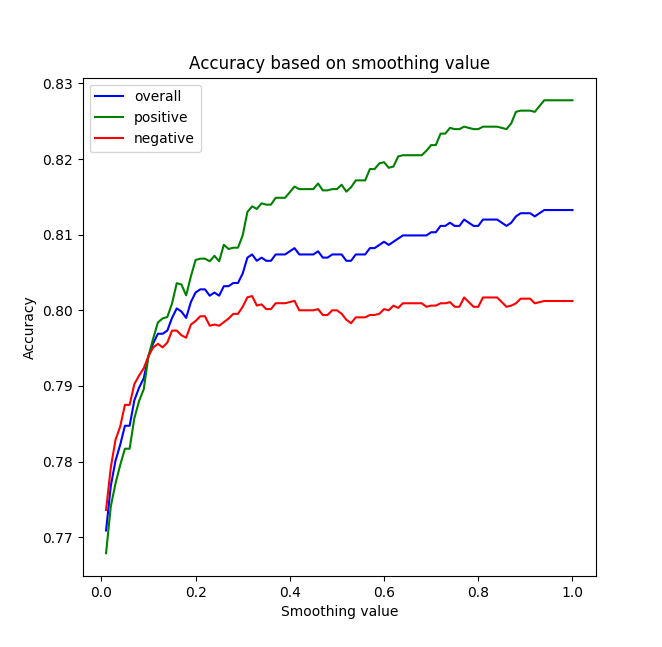
\includegraphics[scale=0.5]{smoothing-average.png}
    \end{figure}
    
    \section{Issues}
    \textcolor{red}{Issues encountered...}
    \section{What would you expand}
    \textcolor{red}{Waht would we expand...}

\end{document}